% THIS IS SIGPROC-SP.TEX - VERSION 3.1
\documentclass{llncs}

% Additional packages
\usepackage{graphicx}
\usepackage{color}
\usepackage{url}
\usepackage{algorithm}
\usepackage[noend]{algpseudocode}
\usepackage{amsmath}
%\usepackage{amsthm}
\usepackage{amsfonts}
\usepackage{amssymb}
\usepackage{booktabs}
\usepackage{multirow}
\usepackage{ifpdf}
% Custom commands
\usepackage{custom_commands}

%\newcommand{\prg}[1]{\paragraph{#1}}
\newcommand{\prg}[1]{\textbf{#1}.}


\newcommand{\Siren}{\textsc{Siren}}
\newcommand{\ReReMi}{\textsc{ReReMi}}

\def\verExample{1}
\def\verE{0}

\begin{document}


\title{Siren: An Interactive Tool for Mining and Visualizing Geospatial Redescriptions}

%\numberofauthors{2} 
\author{
Esther Galbrun\inst{1}
\and
Pauli Miettinen\inst{2}
}

\institute{
  Helsinki Institute for Information Technology,\\
  Department of Computer Science, \\
  University of Helsinki, Finland,\\
  \email{galbrun@cs.helsinki.fi}
\and
  Max Planck Institute for Informatics, \\
  Saarbr{\"u}cken, Germany,\\
  \email{pmiettin@mpi-inf.mpg.de}
}
 
\maketitle
\begin{abstract}
  We present \Siren, an interactive tool for mining and visualizing
  geospatial redescriptions.  Redescription mining is a powerful data
  analysis tool that aims at finding alternative descriptions of the
  same entities.  For example, in biology, an important task is to
  identify the bioclimatic constraints that allow some species to
  survive, that is, to describe geographical regions in terms of both
  the fauna that inhabits them and their bioclimatic conditions.
  
  Using \Siren, users can explore geospatial data of their interest by
  visualizing the redescriptions on a map, interactively edit, extend
  and filter them\footnote{More details about \Siren's features,
    additional screenshots and a demonstration video are available
    online at
    \url{http://www.cs.helsinki.fi/u/galbrun/redescriptors/siren/}.}.

  To demonstrate the use of the tool, we focus on climatic
  niche-finding over Europe, as an example task. However, \Siren\ is by
  no means limited to one particular dataset or application.
\end{abstract}

\section{Introduction}
%\subsubsection{Redescription Mining}
Finding multiple ways to characterize the same entities is a problem
that appears in many areas of science.  In medical sciences, one might
want to find a subset of patients sharing similar symptoms and similar
genes. Describing geographical regions in terms of both their
bioclimatic conditions and the fauna that inhabits them is another
example --- and a task of great importance for biologists.  A 
simple example of a redescription in this setting could state that areas
where Moose live are areas where February's maximum temperature is
between $-10$ and $0$ degrees Celsius and July's maximum temperature
between $12$ and $25$ degrees Celsius. This is actually the
redescription shown in the foreground panel of
Figure~\ref{fig:both_panels}.

However, finding such alternative descriptions of the data
generally requires to manually fix the query on one side before
looking for the best matching query on the other side, using some type
of classification. This typically prevents queries involving more than
one variable to be tested. \emph{Redescription Mining} aims at
solving this tedious task by automatically identifying the best
redescriptions.

More formally, we consider data that contains entities with two sets
of characterizing variables, e.g.\ the fauna and the bioclimatic
conditions. We refer to the two sets of variables as left and right
hand side data, and the queries over them, respectively, as left and
right hand side queries.  The task consists in finding a pair of
queries, one query for both sets of variables, such that both queries
describe (almost) the same set of entities.
Section~\ref{sec:redescription-mining} presents requisite
background information about that problem.

%\note{Two views of redescription mining}
The results of redescription mining, the redescriptions, can be
approached from two points of view. On one hand, by considering the
variables and conditions appearing in the queries, which provide
valuable information in themselves; On the other hand, by studying the
support set of the redescriptions, i.e.\ the subset of entities where
both queries of a redescription hold. When the data is geospatial,
that is, the entities are connected to geographical locations, the
latter approach becomes even more important. A meaningful geospatial
redescription should define coherent areas using expressive
queries. The goal of \Siren\ is to facilitate the analysis of
redescriptions using both of the approaches simultaneously.

Mining data is generally an iterative process, the results obtained at
one step giving rise to hypotheses which will be tested at a further
step, and redescription mining is no exception. Providing means to the
user to easily interact with the mining process greatly improves the
analysis.  When dealing with geospatial data, visualizing the results
on a map is crucial in order to interpret them.  To answer
these needs, we present \Siren, an interactive tool for mining and
visualizing geospatial redescriptions.  

Alternatively, experimenting with \Siren\ provides an efficient way
for unfamiliar users to learn about redescription mining. The
underlying concepts can be easily understood while visualizing the
redescriptions and interacting with the system. Hence, it can also be
used for educational purposes.

% \begin{figure}[hb]
%   \centering
% 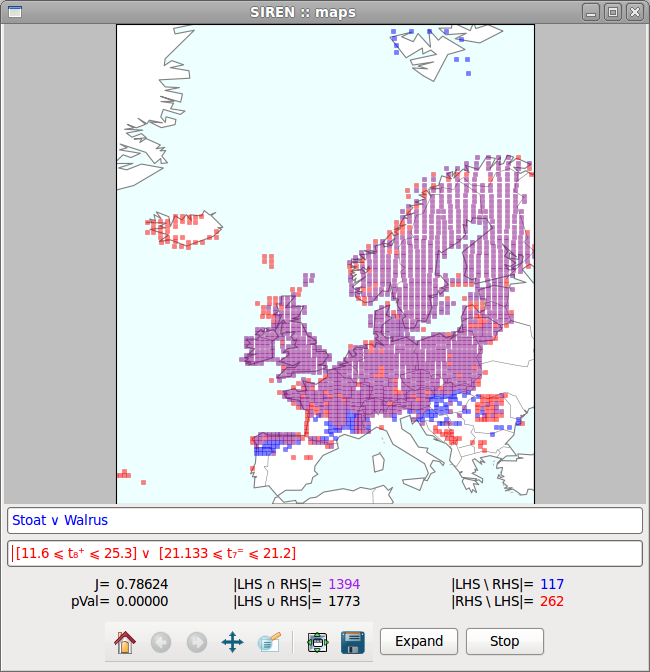
\includegraphics[width=.5\textwidth]{screenshots/siren_map.png}
%   \caption{Map panel, displaying a redescription on a map.}
%   \label{fig:map_panel}
% \end{figure}

\begin{figure*}[t]
  \centering
%%FIG%%
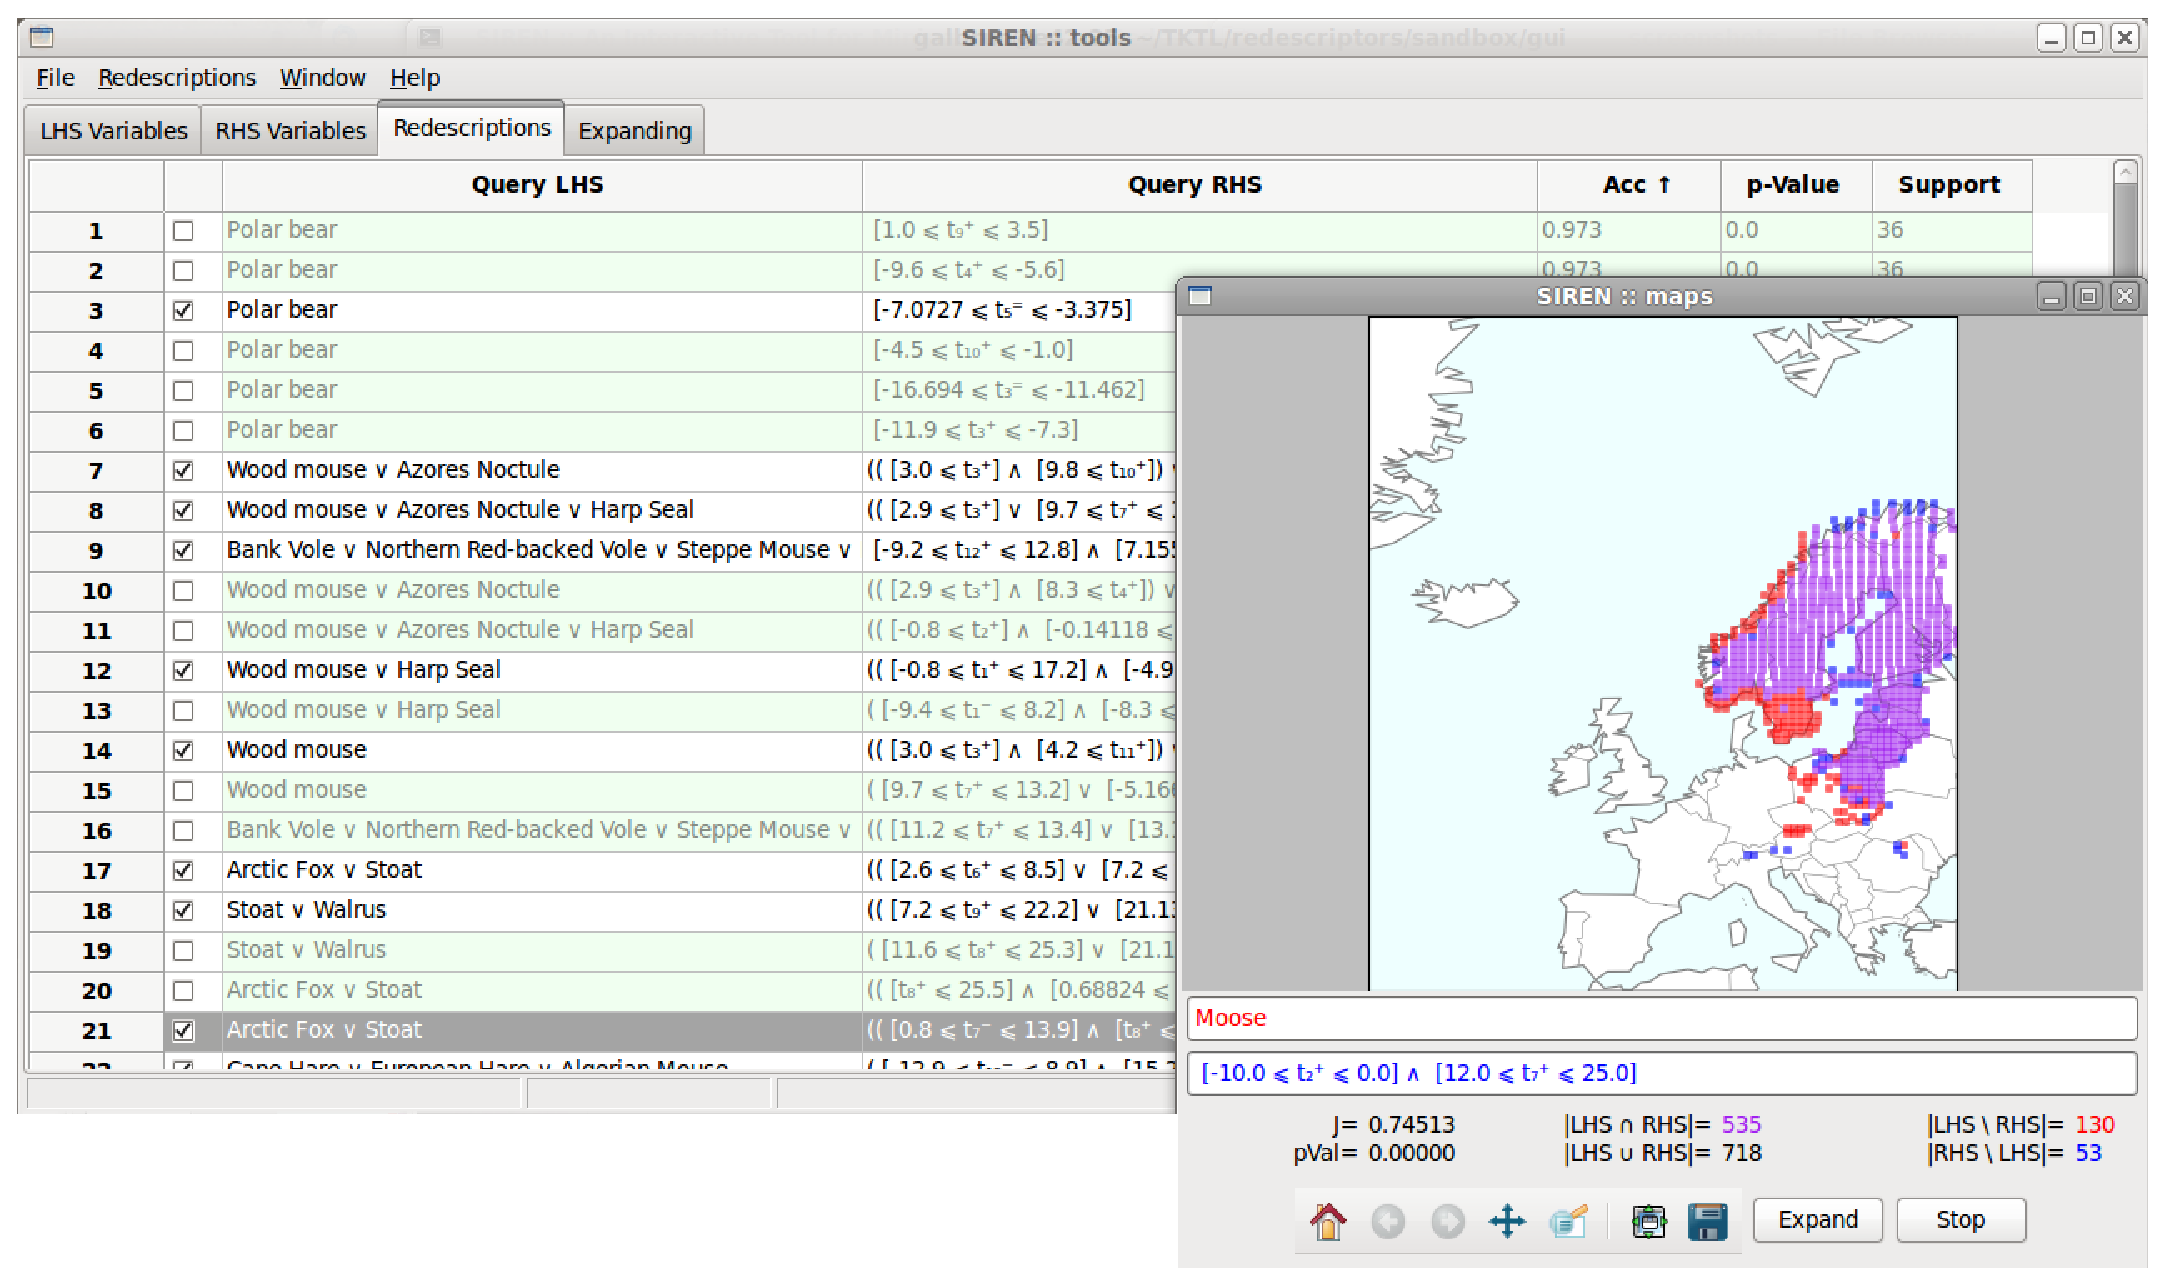
\includegraphics[width=\textwidth]{screenshots/both_panels_02}
  \caption{The \Siren\ interactive mining and visualization tool. The panel in the background contains a list of redescriptions while the foreground panel displays the map of a selected redescription.  In this example, left hand side queries are over fauna while right hand side queries are over monthly bioclimatic conditions, that is, temperatures and precipitation.}
  \label{fig:both_panels}
\end{figure*}

\section{Example applications}
Our main example for demonstrating \Siren\ is an application to
\emph{bioclimatic niche-finding}.

%\prg{Biological niche-finding} 
Indeed, an important problem in biology, niche-finding, is a
particular instance of redescription mining.  The bioclimatic
constraints that must be met for a certain species to survive
constitute that species' bioclimatic envelope, or
niche~\cite{grinnell17niche}.  Finding such envelopes can help, e.g.\
to predict the results of global warming~\cite{pearson03predicting}.
A number of methods, involving regression, neural networks, and
genetic algorithms (see~\cite{soberon05interpretation}) have been
developed over the past ten year to model the bioclimatic envelope,
\textsc{BIOMOD}~\cite{thuiller09biomod} being a good example of a
modelling tool used in this domain.  But to the best of our knowledge,
none of these methods allows automatically finding both the set of
species and their envelope.

We give an example of the application of \Siren\ on this task using data
that describes spatial areas of Europe, squares of side roughly 50
kilometers.  The left hand side data contains information about the
mammals that live in these areas, while the right hand side consists
of bioclimatic variables\footnote{The data comes from two publicly available
datasets: European mammal atlas~\cite{mitchell-jones99atlas} and
Worldclim climate data~\cite{hijmans05very}.}.

% \begin{figure}
%   \centering
% 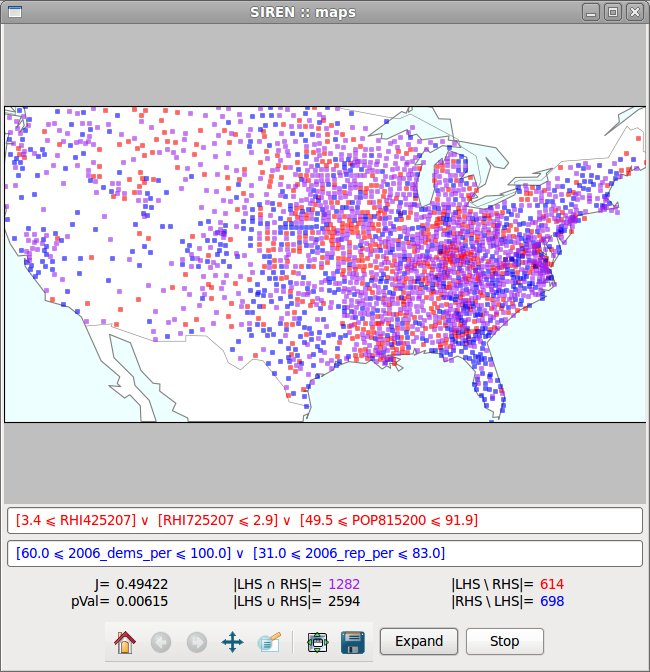
\includegraphics[width=.5\textwidth]{screenshots/siren_map_us_00.jpg}
%   \caption{Map panel, displaying a redescription on a map.}
%   \label{fig:map_panel}
% \end{figure}

Nonetheless, \Siren\ is a flexible tool that can be used with
different datasets from various application domains. For instance, it
could help in sociological studies, with the exploration of
statistical and political data. On the web page, we outline a usage scenario based on census
statistics and electoral campaign funding of U.S. continental counties, as an alternative example.

% \footnote{The data has been gathered
%   from two public websites: FedStats (\url{http://www.fedstats.gov/})
%   and Open Secrets (\url{http://www.opensecrets.org/elections/}).}.


\section{Use-case scenario}
\label{sec:scenarios}
We exemplify the usage of \Siren\ by going through a generic work-flow of
mining geospatial redescriptions, detailing typical steps in the process.  A screenshot of the system,
displaying a list of redescriptions with one
particular redescription plotted on a map is shown in
Figure~\ref{fig:both_panels}.

\prg{Initial redescription mining} A natural starting point for the
analysis of any given data is to use a redescription mining algorithm
to find an initial set of redescriptions.
This can be done withing \Siren{} by running the extension mechanism on an empty redescription.
Then starts the interaction with \Siren.

 
\prg{Extending a redescription} Sometimes the user wants to focus only
on one of the queries, on some particular variable of interest or on a
part of an existing redescription.  \Siren\ allows the user to
automatically extend a given redescription, i.e.\ let the algorithm
add new literals to the queries to make the redescription as accurate
as possible.
% (see Fig.~\ref{fig:extending}). 

The extension mechanism of \Siren\ is based on the beam search
implemented in the \ReReMi\ algorithm~\cite{galbrun11black}. In this case, the intermediate redescriptions
explored during the search are returned at each step, allowing to study
more specific alternative extensions to a redescription that were discarded from the beam
because they were not among the best extensions at some point of the search.

In the climatic niche-finding task, for instance, we might select a
species, say, the Southwestern Water Vole and look for best extensions
starting from that single variable.  Returned extensions can be
visualized side by side and compared as shown in
Figure~\ref{fig:comparison}. Here, the best found extension has
accuracy $0.665$ (per Jaccard coefficient):
\begin{equation*}
%\footnotesize
\begin{array}{l}
\text{Southwestern Water Vole }\lor\text{ Gray Dwarf Hamster }\lor\text{ Savi's Pine Vole }\\[1mm]
\quad\lor\text{ Mediterranean Monk Seal}\\[3mm]
[11.2 \leq t_{3}^{+}] \land  [0.51 \leq t_{1}^{=} \leq 11.333]\land  [42.75 \leq p_{10}^{=} \leq 131.81] \\[1mm]
\quad\land [50.556 \leq p_{11}^{=} \leq 176.75],
\end{array}
\end{equation*}

This redescription indicates that areas where any of the four
species lives correspond to areas where the maximum temperature in
March is above $11.2$ degrees Celsius, the average temperature in January
between $0.51$ and $11.333$ degrees Celsius and the average precipitations in
October and November range from $42.75$ to $131.81$ millimeters and from $50.556$ to $176.75$ millimeters, respectively.


% (see Figure~\ref{fig:extending})
% \begin{figure}
%   \centering
% 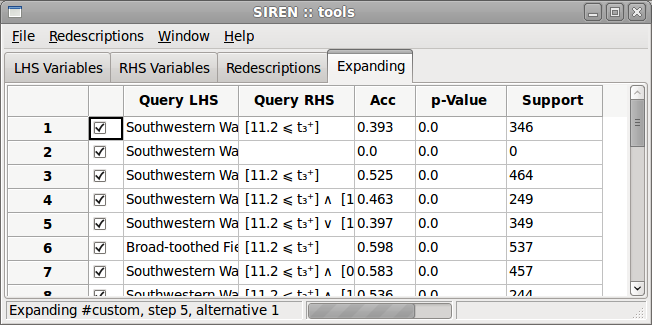
\includegraphics[width=0.5\textwidth]{screenshots/extending.png}
%   \caption{Tool panel. Intermediates results found during the extension of a redescription.}
%   \label{fig:extending}
% \end{figure}

\begin{figure}
  \centering
%%FIG%%
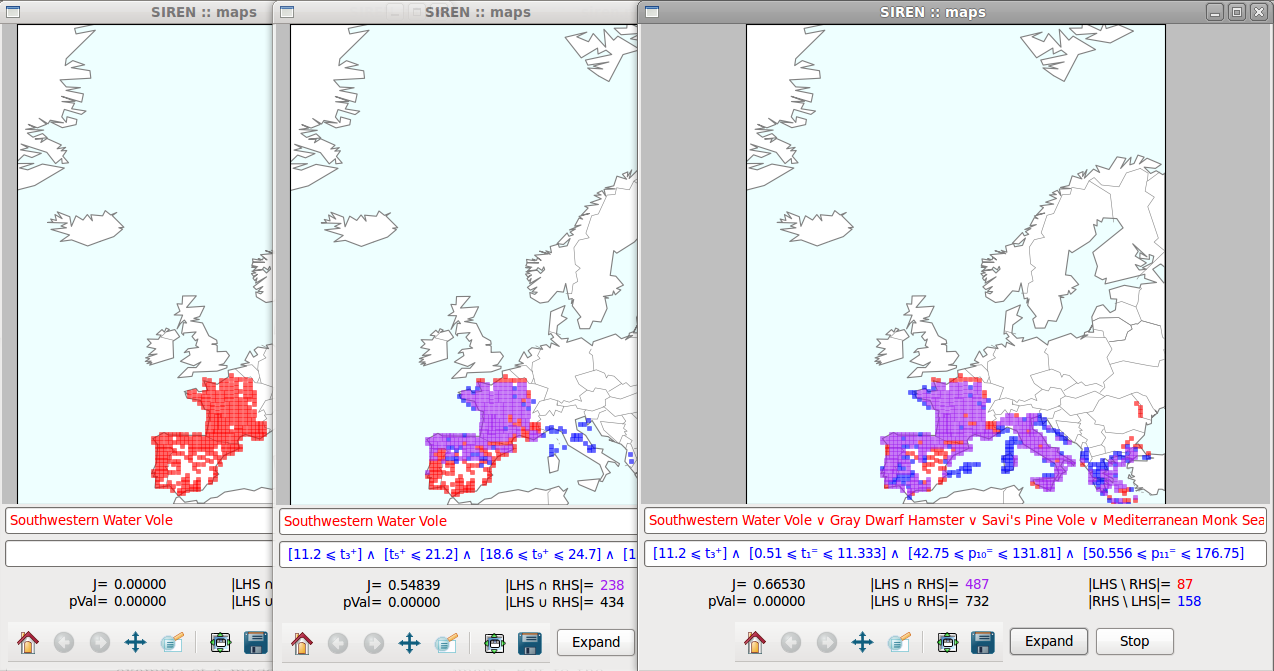
\includegraphics[width=0.7\textwidth]{screenshots/comparison}
  \caption{Several map panels. Comparing intermediate extensions automatically generated for a chosen starting variable. Red, blue and purple represents areas where only the left hand side query holds, only the right hand side query holds and where both queries hold, respectively.}
  \label{fig:comparison}
\end{figure}

\prg{Editing a redescription} It is typical that the user wants to
edit some of the obtained redescriptions. For example, some results
might be overly complex, or have exceedingly precise boundaries for
numerical variables. The user can easily select a redescription to
modify, open it in a map panel and edit it. Boundaries can be altered,
literals added or removed. \Siren\ updates the map and important
statistics (accuracy, $p$-value, etc.) of the redescription, allowing
the user to see the effects of the modifications immediately and
verify, e.g.\ whether the new redescription would still be acceptably
accurate.

Continuing with our example above, we might want to reduce the
precision of the climatic constraints to integers. We could edit the
query as follows:
\begin{equation*}
%\footnotesize
\begin{array}{l}
[11 \leq t_{3}^{+}] \land  [0 \leq t_{1}^{=} \leq 12]%\\[1mm]
%\quad
\land  [42 \leq p_{10}^{=} \leq 132] \land [50 \leq p_{11}^{=} \leq 177],
\end{array}
\end{equation*}
and obtain a redescription of slightly decreased accuracy. % of $0.659$.

\prg{Using subsets of variables} 
\Siren\ allows the user to specify variables to temporarily 
avoid when extending or mining redescriptions.

For example, when two variables are highly
correlated, several redescriptions might contain them
both. The user, however, might want to consider
redescriptions with only one of these variables, not
both. \Siren\ makes that simple: the user only has to select a
redescription, remove the unwanted variable from the
redescription and unselect it from the list of variables, then extend the
redescription again. 

Alternatively, in our running example, we might want to force the
algorithm to search alternative redescriptions that do not involve any
 precipitation. For that purpose, we simply unselect all such
variables before running the extension anew. We will obtain the best
extensions containing only temperatures in the bioclimatic query, such
as the following redescription of accuracy $0.653$:
\begin{equation*}
%\footnotesize
\begin{array}{l}
\text{Southwestern Water Vole }\lor\text{ Cape Hare }\lor\text{ Savi's Pine Vole }\\[1mm]
\quad\lor\text{ Mediterranean Monk Seal}\\[3mm]
( [11.2 \leq t_{3}^{+}] \land  [20.1 \leq t_{7}^{+} \leq 32.9] %\\[1mm] 
%\quad 
\land  [0.51 \leq t_{1}^{=} \leq 11.333]) \lor  [34.0 \leq t_{8}^{+}].
\end{array}
\end{equation*}

Note that this redescription was not returned previously since the
beam search focused on better ones involving precipitation variables.

% \begin{figure}
%   \centering
% 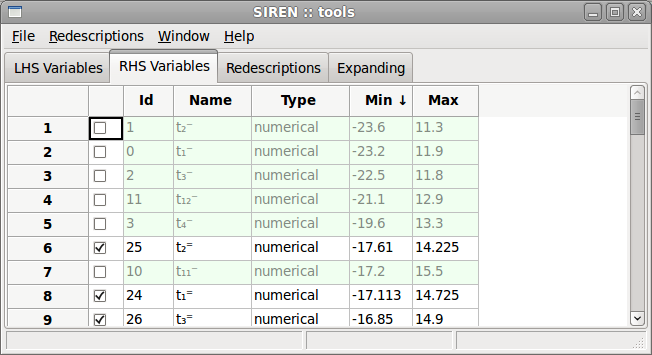
\includegraphics[width=.5\textwidth]{screenshots/variables_05.png}
%   \caption{Tool panel, uselecting variables.}
%   \label{fig:map_panel}
% \end{figure}

% \begin{figure}
%   \centering
% 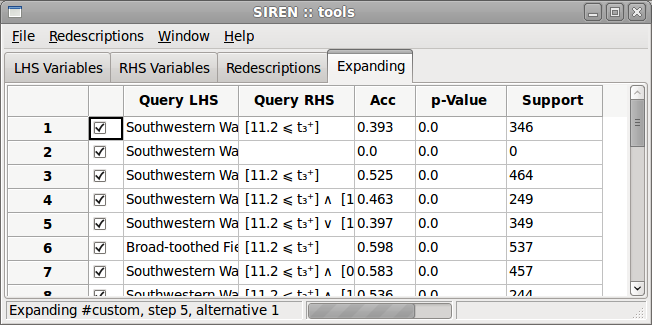
\includegraphics[width=0.5\textwidth]{screenshots/extending.png}
%   \caption{Tool panel, extending a redescription.}
%   \label{fig:extending}
% \end{figure}


\prg{Filtering redundant redescriptions}
\label{sec:filt-redund-redescr}
It is common to see a set of redescriptions that cover approximately
the same area even if they have (somewhat) different sets of
variables.  Indeed, redescriptions belong to the family of local
patterns, with each individual pattern independently describing a
subset of the data. Mining local patterns typically returns redundant
results that require filtering.  In such cases, it is important to be
able to recognize and remove redundant redescriptions, i.e.\
redescriptions that do not convey significant new information, lest
the user be overwhelmed with the number of found
redescriptions. Again, \Siren\ allows automatic filtering of redundant
redescriptions. The user can select a redescription and ask
\Siren\ either to filter out all redescriptions that are redundant
with respect to the selected one, or to go through the whole list of
redescriptions filtering out all redescriptions that are redundant
with respect to some earlier-encountered (i.e.\ better)
redescription. Naturally, the decisions made by
\Siren\ can be reverted whenever the user wishes to.

For instance, the results returned during the extension
mentioned previously may contain many redundant redescriptions found
at different steps. We can easily sort them, e.g.\ by accuracy, select
one of interest and filter all the following results redundant with respect to it.

% \begin{figure}
%   \centering
% 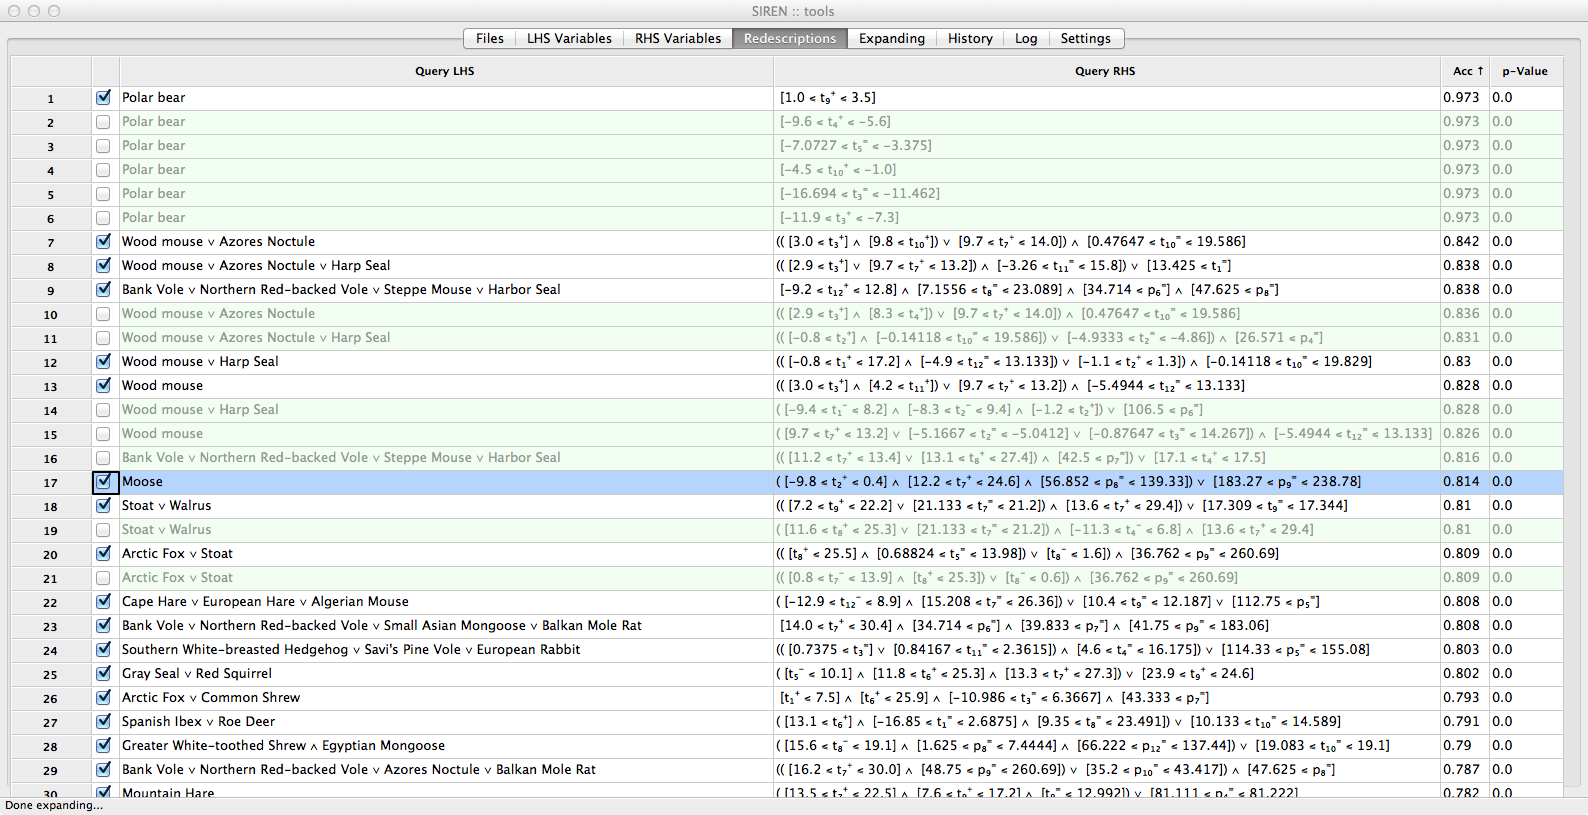
\includegraphics[width=.5\textwidth]{screenshots/redescriptions.png}
%   \caption{Tool panel, filtering redescriptions.}
%   \label{fig:filtering}
% \end{figure}

\prg{Outputting the results}
\label{sec:outputting-results}
Finally, \Siren\ facilitates the distribution of the results:
redescriptions can be exported in easy-to-read format and the
maps associated to redescriptions can be readily converted to
publication-ready graphics. 

\section{Redescription Mining}
\label{sec:redescription-mining}
Redescription mining aims at simultaneously finding multiple
descriptions of a subset of entities which is not previously
specified.  This is in contrast with other methods like Emerging
Patterns Mining (EPM), Contrast Set Mining (CSM) and Subgroup Discovery
(SD) (see \cite{kralj09supervised} for a unifying survey) or general
classification methods, where target subsets of entities are specified
via labels.  Currently, redescription mining is a purely descriptive
approach, its predictive power remains to be explored.  Since its
introduction in~\cite{ramakrishnan04turning} various algorithms have
been proposed for Boolean redescription mining, based on approaches
including decision
trees~\cite{ramakrishnan04turning,kumar07redescription},
co-clusters~\cite{parida05redescription}, and frequent
itemsets~\cite{gallo08finding}.

At the core of \Siren\ is the \ReReMi\ redescription mining
algorithm. This greedy algorithm uses an efficient on-the-fly
discretization technique to extend redescription mining to categorical
and numerical variables.  Below, we give an outline of the concepts and
algorithms involved. Full details can be found
in the original publication~\cite{galbrun11black}.

We consider Boolean, categorical, and numerical variables, partitioned
into two sets. Boolean variables can be interpreted as a truth value
assignment in a natural way.  For categorical and real-valued
variables, truth value assignments are induced by relations $[v=c]$
and $[a \leq v \leq b]$, respectively, where $c$ is some category and
$[a, b]$ an interval.  These truth assignments and their negations
constitute \emph{literals} which can be combined using the Boolean
operators $\land$ (and) and $\lor$ (or) to form \emph{queries}.  Then,
a redescription is simply a pair of queries over variables from the
two sets.  The support of a query is the subset of entities for which
the query holds true.  The \emph{accuracy} of a redescription is
measured by the \emph{Jaccard coefficient} of the supports of its two
queries; \pValue{}s indicating how likely it is to observe such an
overlap for independent queries can be used to reject uninteresting
redescriptions.

% The search space of all Boolean formulae is too huge to be manageable.
% Therefore, we need to restrict ourselves to a subset of formulae that
% provides a good compromise between expressive power, difficulty of the
% search, and interpretability.
% For this purpose, we consider queries that can be parsed in linear
% order, without trees, and allow every variable to appear only once.
% For example, $(a \lor b) \land \lnot c$ is an acceptable query, but
% $(a \land b) \lor (c \land d)$ is not. Yet, the search space remains
% exponential and we still resort to a heuristic pruning during the
% search.
We use a strategy similar to beam-search to explore the
solution space.  The basic idea is to construct queries bottom-up,
starting from singleton redescriptions (i.e.\ both queries contain
only one literal) and progressively extending them by appending
operators and literals. %  For example, we could start with a pair $(a,
% \lnot b)$, and try to extend it to $(a\land c, \lnot b)$, $(a \lor c,
% \lnot b)$, $(a \land \lnot c, \lnot b)$, etc.
After evaluating all
possible one-step extensions, we select the best candidates and extend
them in turn. This process stops when no new redescription can
be generated.

% We exploit some
% simple observations to make the computation of accuracy more
% efficient. This allows to evaluate candidates faster, especially
% extensions with non-Boolean variables.
% We compute a \pValue{} that represents the probability that two random
% queries with marginal probabilities (i.e.\ the fraction of entities
% supporting them) equal to those of $q_\iLHS$ and $q_\iRHS$ have an
% intersection equal to or larger than $\abs{\supp(q_\iLHS,
%   q_\iRHS)}$. This probability uses the binomial distribution. The higher the
% \pValue, the more likely it is to observe such a support for
% independent queries, and the less significant the query. Redescriptions with too high \pValue{} can be discarded.

\section{Implementation details}
\Siren\ and \ReReMi\ are implemented in Python.  The interface is
built with the \texttt{wxPython} Open Source GUI toolkit, ensuring
cross-platform compatibility.  The \texttt{matplotlib} library enables
to generate high quality figures, seamlessly integrated in the
interface.  \Siren\ allows for simple editing of the redescriptions
thanks to flexible parsing of different representations. It can handle
any data provided in a compatible format.

The formulation of redescription mining presented here assumes that
the describing variables are partitioned into two sets apriori, and
looks for a pairs of queries over these two sets, respectively.
However, this can be naturally adapted to settings with a single set
of describing variables.  One might then search for pairs of queries,
with the constraint that the two subsets of variables appearing in the
queries of any redescription be disjoint or enable the user to
interactively determine the split between the variables.

\section{Analysis of the functionalities}
In this section, we analyse from a high-level perspective the dynamic interation functionalities of \Siren. We discuss functionalities currently integrated into the tool as well as speculate about useful functionalities that could be included in the future.
As a basis for our discussion, we use the taxonomy of interations for visual analytics proposed by Heer and Shneiderman~\cite{Heer:2012:IDV:2133806.2133821}.

\begin{description}
\item[Data and View Specification]~
\begin{description}
\item[Visualize] Plotting redescriptions on a map. Maps are the most natural way of visualizing geospatial data. (Possibly visualize several redescriptions on one map simultaneously? Advantages/Drawbacks?)
\item[Filter] Filter by variables (literal?) to exclude or require them, by geographical locations, statistics.
\item[Sort] Sort the redescription based on similar criteria as filtering. Filter vs. Sort: show/hide vs. color code, e.g. shades of grey. Filtering can be similar to a strict thresholded sorting.
\item[Derive] Introduce new variables as aggregate  (how close does it come to new query operators). Modify the split between variables. Have only one set of variables among which one can specify \emph{incompoatibilities} and \emph{exclusions}, i.e. variables that cannot appear in the same query or in the same redescription respectively (That takes the form of a graph with two types of edges).
\end{description}
\item[View Manipulation]~
\begin{description}
\item[Select] Select a redescription (possibility to select a several redescriptions at once? What for?) Specifying the bounds for real valued variables. Click or hover on a dot in the map to get more information about the state of the variables and what makes a query hold or not in that particular location.
\item[Navigate] Shows the redescription over the whole area first, allows to zoom and pan. (Highlight the most relevant redescriptions to the currently zoomed on area, i.e. doing some filtering.) Keep an overview map in a corner of each map, maybe that's somewhat of an overkill, or have one general view with rectangles corresponding to zooms in the currently other opened maps.
\item[Coordinate] When editing real-valued variable, show a scatter plot of the entities based on the values of the variable (and geographical proximity for y axis?) with colors indicating the current status of the rest of the query for each entity and provide sliders to set the bounds of the variable. Update the map view based accordingly. Update map(s) and list(s) on edits. Indicate in the list redescriptions which are currently displayed. Set a default zoom to which one can tie and untie map windows, zooming and panning in one window tied to that default zoom is reflected in other tied windows. One can choose whether map windows are created tied to the zoom or not, in the first case they would be created with the current default zoom else display the whole area.
\item[Organize] Open maps (and new redescription lists) in different windows (using the system's tiling if there is one), or in detachable tabs.
\end{description}
\item[Process and Provenance]~
\begin{description}
\item[Record] Allow to save the current status, i.e. all current redescriptions, opened panels, maps, selected redescription and potentialy full history. Record the interaction history. Support redo and undo (only for edits or also for plotting, zooming, sorting, etc.). Turn the interaction history into editable/parameterizable macros. Find the shortest events sequence to reach the current status from initialization.
\item[Annotate] Allow to add comments to the interaction history and macros, with annotable screen shots of the current window of interest or link to objects in the current environment (redescriptions, entities, groups of entities, variables, literals, etc.) Allow to structure the history and macros into logical blocks. 
\item[Share] Easy export/import of macros, redescriptions lists, maps, possibly with comments and annotations and possibly individual events in the interaction history (requires specification of pre-requisites).
\item[Guide] Give a clear name to and provide feedback for each action. Explain why an action might not be applicable at a certain point. Provide example macros with detailed explanations, to be replayed step-by-step. 
\end{description}
\end{description}

\section{Pitfalls}
How to avoid that the user finds what he is looking for and only that?
That is, a tool not to explore data and formulate new hypotheses, but to find arguments to support pre-existing theories?

Data mining is an iterative process of refining hypotheses. The tool generates hypotheses about the data, here in the form of redescriptions. Then the user is able to select one, edit it, let the tool expand it. When satisfied with it, the user can remove redundant hypotheses and move on to the next one of interest. That is, at some point he is able to state that now, the information provided by the current hypothesis is admitted to be known, i.e. included in the knowledge and further hypotheses that does not add any information to that knowledge should be discarded.

It is possible to evaluate a completely hand-crafted redescription. Is this a problem? Why?

When considering a redescription, one should always keep in mind the assumptions attached it. For example, if some variables where disabled or if the focus was put on some particular area when it was generated.

When considering an edited redescription (and mabye also in any case), the tool should allow to evaluate the interestingness of the redescription (using \pValue{}s or randomization techniques). The tool should also suggest other related results, concerning the same area, the same variables or having similar statistics, to provide context to that redescription and challenge the current hypothesis.

What is the difference between generating hypotheses from the data versus backing hypotheses with the data.

In the mining process, one starts with a question, which is often implicit, makes an hypothesis to answer it. Then the tool could help look for evidence supporting the hypothesis. Rather, it should help indentify the hypothesis that best answers the question.  

\section{Conclusions}
We present \Siren, a tool for mining geospatial redescriptions. It enables
users to interactively mine, edit and extend redescriptions. It also
features visualization of the redescriptions on a map, a key toward
interpreting the results of geospatial data mining.

We will give chance to the public to experiment with \Siren\ and
together consider how this tool could be used to explore their own geospatial
data and help answer their data analysis need.

\bibliographystyle{abbrv}
%\nocite{*}
\bibliography{bibsiren}  
\end{document}

%%% Local Variables: 
%%% mode: latex
%%% TeX-master: t
%%% End: 
